

\section{Begrüssung}
Ich möchte Eberhardt und euch alle herzlich zu diesem Gottesdienst begrüssen.
\\
Lasst uns beten und dann ein Lied zu ehre Gottes singen, \textit{Nur durch Christus in mir}

\section{Ankündigungen}
\begin{itemize}
    \item Nächster Bibel und Gebetsabend am Donnerstag:
    4.07.2024  RÖMER 8,28-30    ??
    \item Nächster Gottesdienst: 7.07.2024 mit ??
\end{itemize}
Letztes mal habe ich euch einen Flyer mit einem Anlass der Gemeinde Bern gezeigt. Leider habe ich diesen Anlass mit dem Freundestreffen am 15.Sept verwechselt. Am 18.8 ist ein Gemeindefest. Wer will kann da hingehen, aber wir werden nicht geschlossen dahin gehen. Ihr könnt euch gerne Untereinnander Oganisieren. Anders ist es am 15.9.2024 zum Freundestreffen in Bern. Da wollen wir gemeinsam zum Gottesdienst hinfahren.
\section{ Input }
Ich nehme mir öfter mal vor die Bibel von vorne nach hinten durchzulesen, und fange bei 1. Moses oder auch Genesis an. Dann gehts weiter bis Abraham und es fehlt einem plötzlich wieder die Zeit. Aus diesem Grund liest man die ersten paar Kaptiel fleissiger als spätere.

Mir ist aufgefallen wie genial Gott es gemacht hat, dass alle Menschen ihn kennen lernen durften. Jedes Volk auf Erden hat von diesem einen Gott gehört, wie er ist und was er gemacht hat.

Ihr kennt doch diese Namenliste mit den Urmenschen in 1. Moses 5 6 - 32. Ich habe diese schon vor längerer Zeit mal grafisch dargestellt:
\begin{figure}[ht]
	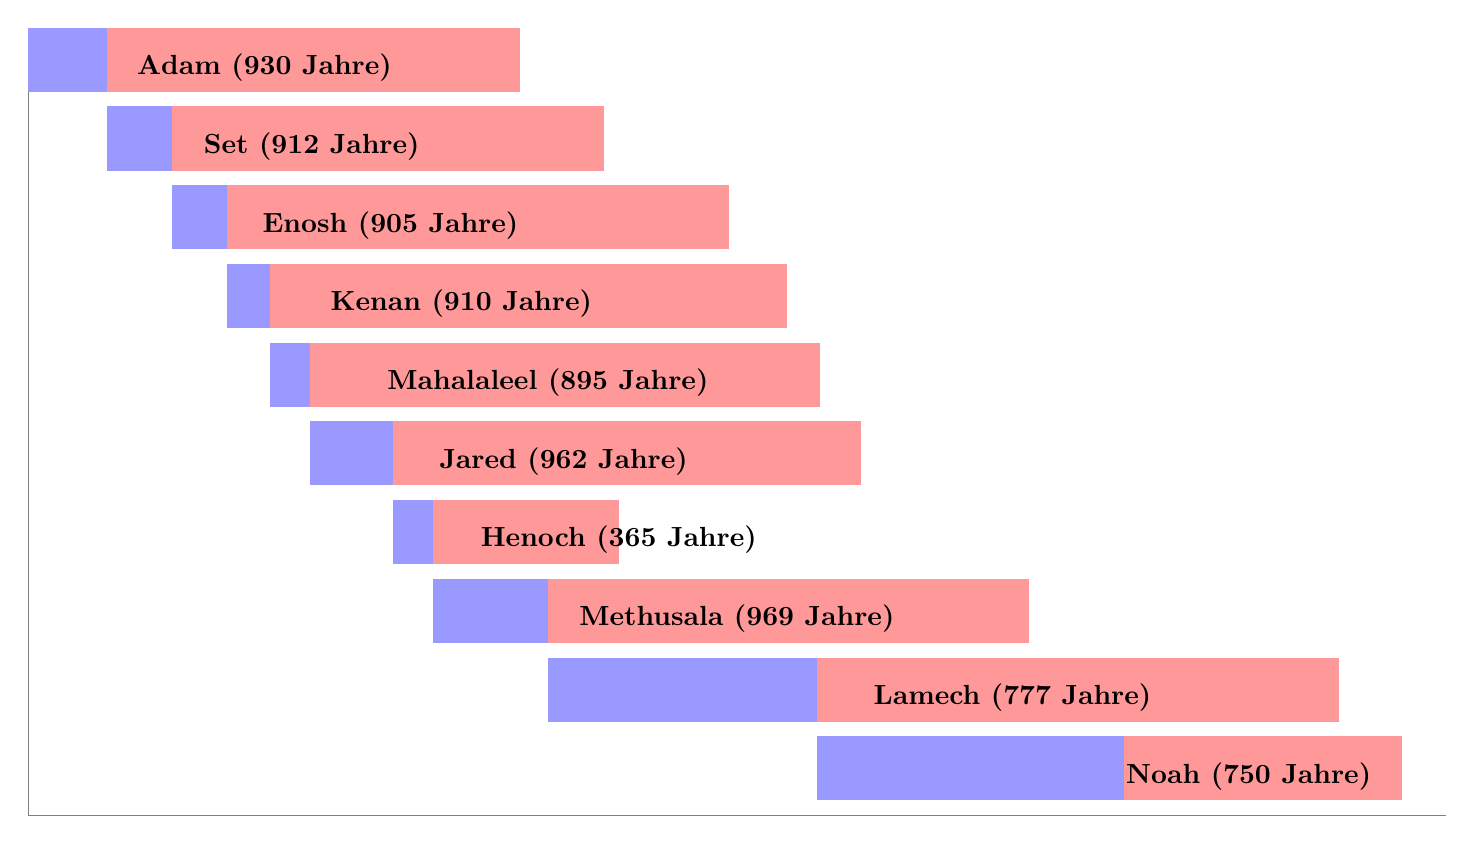
\begin{tikzpicture}
		\draw[gray] (0,0) -- (0mm, 100mm);
		%Adam 130-800 (10.1 - 62.4)
		\filldraw[blue!40] (0,100mm) rectangle(10.1mm,92mm);
		\filldraw[red!40] (10.1mm,100mm) rectangle(62.4mm,92mm) node at (30mm, 92mm) [right, above, black]{\textbf{Adam (930 Jahre)}};
		%Set 105-807 (8.19 - 62.9)
		\filldraw[blue!40] (10.1mm,90mm) rectangle(18.29mm,82mm);
		\filldraw[red!40] (18.29mm,90mm) rectangle(73.0mm,82mm) node at (36mm, 82mm) [right, above, black]{\textbf{Set (912 Jahre)}};
		%Enosch 90 - 815 (7.02 - 63.6)	
		\filldraw[blue!40] (18.29mm,80mm) rectangle (25.31mm,72mm);
		\filldraw[red!40] (25.31mm,80mm) rectangle(88.91mm,72mm) node at (46mm, 72mm) [right, above, black]{\textbf{Enosh (905 Jahre)}};
		%Kenan 70 - 840 (5.46 - 65.52)		
		\filldraw[blue!40] (25.31mm,70mm) rectangle(30.77mm,62mm);
		\filldraw[red!40] (30.77mm,70mm) rectangle(96.29mm,62mm) node at (55mm, 62mm) [right, above, black]{\textbf{Kenan (910 Jahre)}};
		%Mahalaleel 65 - 830 (5.07 - 64.7)
		\filldraw[blue!40] (30.77mm,60mm) rectangle(35.84mm,52mm);
		\filldraw[red!40] (35.84mm,60mm) rectangle(100.54mm,52mm) node at (66mm, 52mm) [right, above, black]{\textbf{Mahalaleel (895 Jahre)}};
		%Jared 162 - 800 (12.6 - 62.4)
		\filldraw[blue!40] (35.84mm,50mm) rectangle(46.44mm,42mm);
		\filldraw[red!40] (46.44mm,50mm) rectangle(105.68mm,42mm) node at (68mm, 42mm) [right, above, black]{\textbf{Jared (962 Jahre)}};
		%Henoch 65 - 300 (5.07 - 23.4)
		\filldraw[blue!40] (46.44mm,40mm) rectangle(51.51mm,32mm);
		\filldraw[red!40] (51.51mm,40mm) rectangle(74.91mm,32mm) node at (75mm, 32mm) [right, above, black]{\textbf{Henoch (365 Jahre)}};
		%Methusalah 187 - 782 (14.58 - 60.99)
		\filldraw[blue!40] (51.51mm,30mm) rectangle(66.09mm,22mm);
		\filldraw[red!40] (66.09mm,30mm) rectangle(127.08mm,22mm) node at (90mm, 22mm) [right, above, black]{\textbf{Methusala (969 Jahre)}};
		%Lamech 182 - 595 (14.19 - 46.41)
		\filldraw[blue!40] (66.09mm,20mm) rectangle(100.28mm,12mm);
		\filldraw[red!40] (100.28mm,20mm) rectangle(166.37mm,12mm) node at (125mm, 12mm) [right, above, black]{\textbf{Lamech (777 Jahre)}};
		% Noah 500 - 450 (39 - 35.1)
		\filldraw[blue!40] (100.28mm,10mm) rectangle(139.28mm,2mm);
		\filldraw[red!40] (139.28mm,10mm) rectangle(174.38mm,2mm) node at (155mm, 2mm) [right, above, black]{\textbf{Noah (750 Jahre)}};

		\draw[gray] (0,0) -- (180mm, 0mm);
	\end{tikzpicture}
	\caption{Lebensjahre bis Noah}
	\label{balken_alter}
\end{figure}
Ob ich glaube dass die Menschen wirklich so alt wurden? Ja, ich glaube es. Es ist eine effektive Art zu wachsen und etwas von Generation zu Generation weiter zu sagen. 

Bei Noah hat dann Gott entschlossen neu anzufangen. Er schickte die Sintflut und alles starben ausser die Bewohner der Arche. Danach hat Gott das Lebenalter begrenzt. Zu beginn war es noch um die 400 Jahre dann 200 Jahre und es ging zurüch auf unsere heutigen 120 Jahre.
\begin{figure}[ht]
	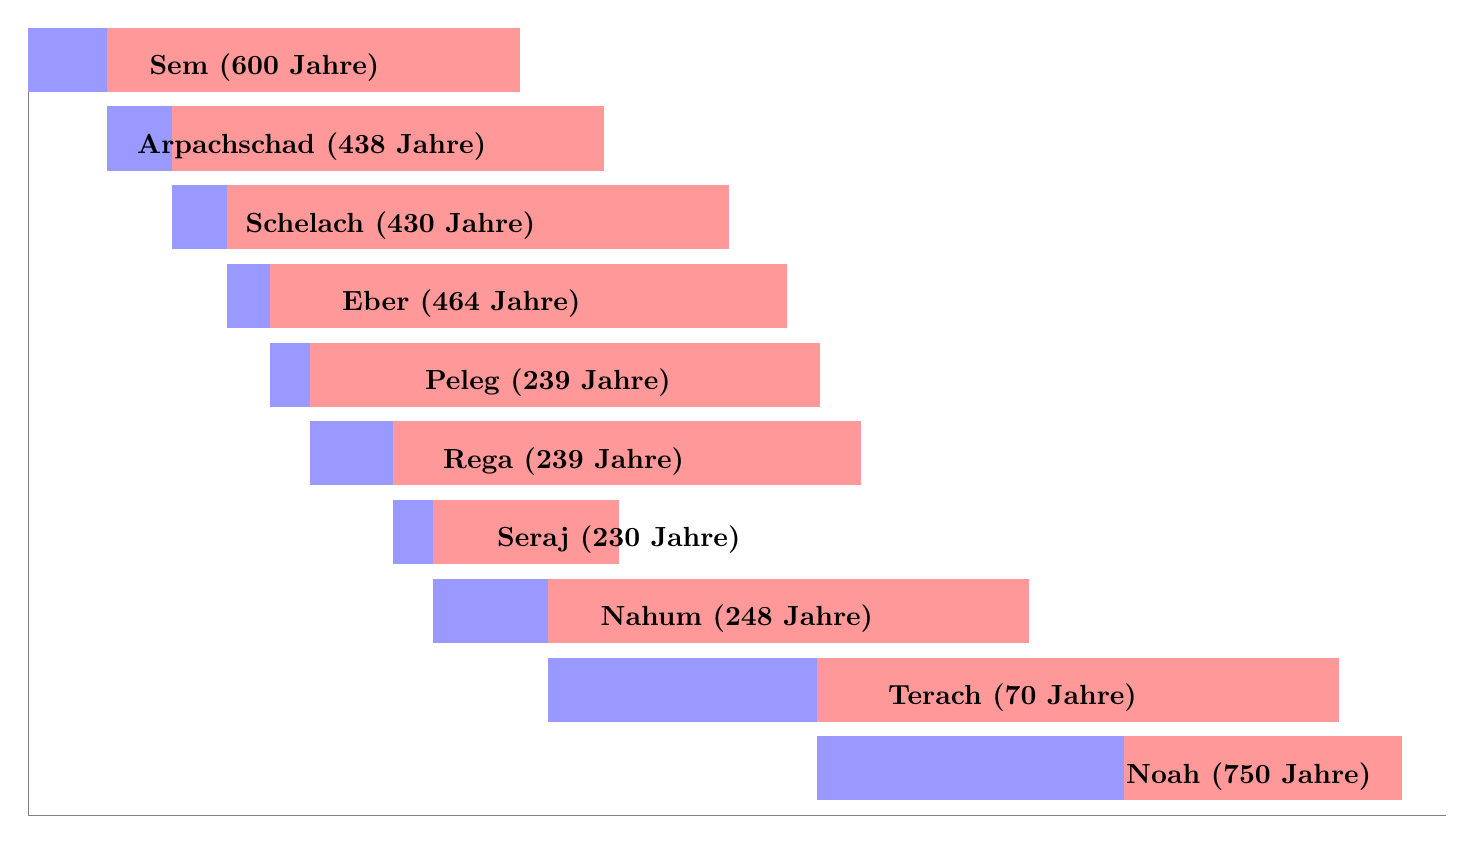
\begin{tikzpicture}
		\draw[gray] (0,0) -- (0mm, 100mm);
		%Sem 35-500 (10.1 - 62.4)
		\filldraw[blue!40] (0,100mm) rectangle(10.1mm,92mm);
		\filldraw[red!40] (10.1mm,100mm) rectangle(62.4mm,92mm) node at (30mm, 92mm) [right, above, black]{\textbf{Sem (600 Jahre)}};
		%Arpachad 35-403 (8.19 - 62.9)
		\filldraw[blue!40] (10.1mm,90mm) rectangle(18.29mm,82mm);
		\filldraw[red!40] (18.29mm,90mm) rectangle(73.0mm,82mm) node at (36mm, 82mm) [right, above, black]{\textbf{Arpachschad (438 Jahre)}};
		%Schelach 30 - 403 (7.02 - 63.6)	
		\filldraw[blue!40] (18.29mm,80mm) rectangle (25.31mm,72mm);
		\filldraw[red!40] (25.31mm,80mm) rectangle(88.91mm,72mm) node at (46mm, 72mm) [right, above, black]{\textbf{Schelach (430 Jahre)}};
		%Eber 34 - 430 (5.46 - 65.52)		
		\filldraw[blue!40] (25.31mm,70mm) rectangle(30.77mm,62mm);
		\filldraw[red!40] (30.77mm,70mm) rectangle(96.29mm,62mm) node at (55mm, 62mm) [right, above, black]{\textbf{Eber (464 Jahre)}};
		%Peleg 30 - 209 (5.07 - 64.7)
		\filldraw[blue!40] (30.77mm,60mm) rectangle(35.84mm,52mm);
		\filldraw[red!40] (35.84mm,60mm) rectangle(100.54mm,52mm) node at (66mm, 52mm) [right, above, black]{\textbf{Peleg (239 Jahre)}};
		%Regu 32 - 207 (12.6 - 62.4)
		\filldraw[blue!40] (35.84mm,50mm) rectangle(46.44mm,42mm);
		\filldraw[red!40] (46.44mm,50mm) rectangle(105.68mm,42mm) node at (68mm, 42mm) [right, above, black]{\textbf{Rega (239 Jahre)}};
		%Seray 30 - 200 (5.07 - 23.4)
		\filldraw[blue!40] (46.44mm,40mm) rectangle(51.51mm,32mm);
		\filldraw[red!40] (51.51mm,40mm) rectangle(74.91mm,32mm) node at (75mm, 32mm) [right, above, black]{\textbf{Seraj (230 Jahre)}};
		%Nahor 29 - 119 (14.58 - 60.99)
		\filldraw[blue!40] (51.51mm,30mm) rectangle(66.09mm,22mm);
		\filldraw[red!40] (66.09mm,30mm) rectangle(127.08mm,22mm) node at (90mm, 22mm) [right, above, black]{\textbf{Nahum (248 Jahre)}};
		%Terach 70 - 135 (14.19 - 46.41)
		\filldraw[blue!40] (66.09mm,20mm) rectangle(100.28mm,12mm);
		\filldraw[red!40] (100.28mm,20mm) rectangle(166.37mm,12mm) node at (125mm, 12mm) [right, above, black]{\textbf{Terach (70 Jahre)}};
		% Abraham 165
		\filldraw[blue!40] (100.28mm,10mm) rectangle(139.28mm,2mm);
		\filldraw[red!40] (139.28mm,10mm) rectangle(174.38mm,2mm) node at (155mm, 2mm) [right, above, black]{\textbf{Noah (750 Jahre)}};

		\draw[gray] (0,0) -- (180mm, 0mm);
	\end{tikzpicture}
	\caption{Lebensjahre nach Noah bis Abraham}
	\label{balken_alter}
\end{figure}

Darum singen wir jetzt das Lied \textit{Nimm mein Leben}
Danach nimmt Oswald die Schriftlesung vor zur Predigt vor.

\section{Predigt}
Das Wort wird von Nathanael verkündigt.
\\
\\
\textbf{Nach der Predigt}\\
Nathanel vielen Dank für deine Worte...

Wir singen unser letztes Lied \textit{Du bist mein Ziel mein Gott}

\section{Abschluss}
(Philipper 4 20.23):
\begin{bibeltext}{Sch2}{Phil}{4:20.23}
Unser Gott und Vater aber sei die Herrlichkeit von Ewigkeit zu Ewigkeit!
Die Gnade des Herrn Jesus Christus sei mit eurem Geist!
\end{bibeltext}
Amen! Maranatha, der Herr komme bald!
